\documentclass[12pt letter]{report}
%%%%%%%%%%%%%%%%%%%%%%%%%%%%%%%%%
% PACKAGE IMPORTS
%%%%%%%%%%%%%%%%%%%%%%%%%%%%%%%%%


\usepackage[tmargin=2cm,rmargin=1in,lmargin=1in,margin=0.85in,bmargin=2cm,footskip=.2in]{geometry}
\usepackage{amsmath,amsfonts,amsthm,amssymb,mathtools}
\usepackage[varbb]{newpxmath}
\usepackage{xfrac}
\usepackage[makeroom]{cancel}
\usepackage{mathtools}
\usepackage{bookmark}
\usepackage{enumitem}
\usepackage{hyperref,theoremref}
\hypersetup{
  pdftitle={Assignment},
  colorlinks=true, linkcolor=doc!90,
  bookmarksnumbered=true,
  bookmarksopen=true
}
\usepackage[most,many,breakable]{tcolorbox}
\usepackage{xcolor}
\usepackage{varwidth}
\usepackage{varwidth}
\usepackage{etoolbox}
%\usepackage{authblk}
\usepackage{nameref}
\usepackage{multicol,array}
\usepackage{tikz-cd}
\usepackage[ruled,vlined,linesnumbered]{algorithm2e}
\usepackage{comment} % enables the use of multi-line comments (\ifx \fi) 
\usepackage{import}
\usepackage{xifthen}
\usepackage{pdfpages}
\usepackage{transparent}
\usepackage{xcolor,colortbl,array,amssymb}
\usepackage{venndiagram}
\usepackage{listings}
\usepackage{fontspec}

\setmainfont{LibertinusSerif}[
  Extension = .otf,
  Path = /usr/share/fonts/libertinus/,
  UprightFont = *-Regular,
  ItalicFont = *-Italic,
  BoldFont = *-Bold,
  BoldItalicFont = *-BoldItalic,
]

\setmonofont{CaskaydiaCoveNerdFontMono}[
  Extension = .ttf,
  Path = /usr/share/fonts/TTF/,
  UprightFont = *-Regular,
  ItalicFont = *-Italic,
  BoldFont = *-Bold,
  BoldItalicFont = *-BoldItalic,
]

\definecolor{listing-background}{HTML}{F7F7F7}
\definecolor{listing-rule}{HTML}{B3B2B3}
\definecolor{listing-numbers}{HTML}{B3B2B3}
\definecolor{listing-text-color}{HTML}{000000}
\definecolor{listing-keyword}{HTML}{435489}
\definecolor{listing-keyword-2}{HTML}{1284CA} % additional keywords
\definecolor{listing-keyword-3}{HTML}{9137CB} % additional keywords
\definecolor{listing-identifier}{HTML}{435489}
\definecolor{listing-string}{HTML}{00999A}
\definecolor{listing-comment}{HTML}{8E8E8E}

\lstdefinestyle{eisvogel_listing_style}{
language         = java,
xleftmargin      = 0.6em,
framexleftmargin = 0.4em,
backgroundcolor  = \color{listing-background},
basicstyle       = \color{listing-text-color}\linespread{1.0}%
\lst@ifdisplaystyle%
\fi\ttfamily{},
breaklines       = true,
frame            = single,
framesep         = 0.19em,
rulecolor        = \color{listing-rule},
frameround       = ffff,
tabsize          = 4,
numberstyle      = \color{listing-numbers},
aboveskip        = 1.0em,
belowskip        = 0.1em,
abovecaptionskip = 0em,
belowcaptionskip = 1.0em,
keywordstyle     = {\color{listing-keyword}\bfseries},
keywordstyle     = {[2]\color{listing-keyword-2}\bfseries},
keywordstyle     = {[3]\color{listing-keyword-3}\bfseries\itshape},
sensitive        = true,
identifierstyle  = \color{listing-identifier},
commentstyle     = \color{listing-comment},
stringstyle      = \color{listing-string},
showstringspaces = false,
escapeinside     = {/*@}{@*/}, % Allow LaTeX inside these special comments
literate         =
  {á}{{\'a}}1 {é}{{\'e}}1 {í}{{\'i}}1 {ó}{{\'o}}1 {ú}{{\'u}}1
{Á}{{\'A}}1 {É}{{\'E}}1 {Í}{{\'I}}1 {Ó}{{\'O}}1 {Ú}{{\'U}}1
{à}{{\`a}}1 {è}{{\`e}}1 {ì}{{\`i}}1 {ò}{{\`o}}1 {ù}{{\`u}}1
{À}{{\`A}}1 {È}{{\`E}}1 {Ì}{{\`I}}1 {Ò}{{\`O}}1 {Ù}{{\`U}}1
{ä}{{\"a}}1 {ë}{{\"e}}1 {ï}{{\"i}}1 {ö}{{\"o}}1 {ü}{{\"u}}1
{Ä}{{\"A}}1 {Ë}{{\"E}}1 {Ï}{{\"I}}1 {Ö}{{\"O}}1 {Ü}{{\"U}}1
{â}{{\^a}}1 {ê}{{\^e}}1 {î}{{\^i}}1 {ô}{{\^o}}1 {û}{{\^u}}1
{Â}{{\^A}}1 {Ê}{{\^E}}1 {Î}{{\^I}}1 {Ô}{{\^O}}1 {Û}{{\^U}}1
{œ}{{\oe}}1 {Œ}{{\OE}}1 {æ}{{\ae}}1 {Æ}{{\AE}}1 {ß}{{\ss}}1
{ç}{{\c c}}1 {Ç}{{\c C}}1 {ø}{{\o}}1 {å}{{\r a}}1 {Å}{{\r A}}1
{€}{{\EUR}}1 {£}{{\pounds}}1 {«}{{\guillemotleft}}1
{»}{{\guillemotright}}1 {ñ}{{\~n}}1 {Ñ}{{\~N}}1 {¿}{{?`}}1
{…}{{\ldots}}1 {≥}{{>=}}1 {≤}{{<=}}1 {„}{{\glqq}}1 {“}{{\grqq}}1
{”}{{''}}1
}
\lstset{style=eisvogel_listing_style,
  numbers=left}

%
% Java (Java SE 12, 2019-06-22)
%
\lstdefinelanguage{Java}{
  morekeywords={
      % normal keywords (without data types)
      abstract,assert,break,case,catch,class,continue,default,
      do,else,enum,exports,extends,final,finally,for,if,implements,
      import,instanceof,interface,module,native,new,package,private,
      protected,public,requires,return,static,strictfp,super,switch,
      synchronized,this,throw,throws,transient,try,volatile,while,
      % var is an identifier
      var
    },
  morekeywords={[2] % data types
      % primitive data types
      boolean,byte,char,double,float,int,long,short,
      % String
      String,
      % primitive wrapper types
      Boolean,Byte,Character,Double,Float,Integer,Long,Short
      % number types
      Number,AtomicInteger,AtomicLong,BigDecimal,BigInteger,DoubleAccumulator,DoubleAdder,LongAccumulator,LongAdder,Short,
      % other
      Object,Void,void
    },
  morekeywords={[3] % literals
      % reserved words for literal values
      null,true,false,
    },
  sensitive,
  morecomment  = [l]//,
  morecomment  = [s]{/*}{*/},
  morecomment  = [s]{/**}{*/},
  morestring   = [b]",
  morestring   = [b]',
}

\lstdefinelanguage{XML}{
  morestring      = [b]",
  moredelim       = [s][\bfseries\color{listing-keyword}]{<}{\ },
  moredelim       = [s][\bfseries\color{listing-keyword}]{</}{>},
  moredelim       = [l][\bfseries\color{listing-keyword}]{/>},
  moredelim       = [l][\bfseries\color{listing-keyword}]{>},
  morecomment     = [s]{<?}{?>},
  morecomment     = [s]{<!--}{-->},
  commentstyle    = \color{listing-comment},
  stringstyle     = \color{listing-string},
  identifierstyle = \color{listing-identifier}
}


\newcommand\mycommfont[1]{\footnotesize\ttfamily\textcolor{blue}{#1}}
\SetCommentSty{mycommfont}
\newcommand{\incfig}[1]{%
  \def\svgwidth{\columnwidth}
  \import{./figures/}{#1.pdf_tex}
}

\usepackage{tikzsymbols}
\renewcommand\qedsymbol{$\Laughey$}


%\usepackage{import}
%\usepackage{xifthen}
%\usepackage{pdfpages}
%\usepackage{transparent}


%%%%%%%%%%%%%%%%%%%%%%%%%%%%%%
% SELF MADE COLORS
%%%%%%%%%%%%%%%%%%%%%%%%%%%%%%



\definecolor{myg}{RGB}{56, 140, 70}
\definecolor{myb}{RGB}{45, 111, 177}
\definecolor{myr}{RGB}{199, 68, 64}
\definecolor{mytheorembg}{HTML}{F2F2F9}
\definecolor{mytheoremfr}{HTML}{00007B}
\definecolor{mylenmabg}{HTML}{FFFAF8}
\definecolor{mylenmafr}{HTML}{983b0f}
\definecolor{mypropbg}{HTML}{f2fbfc}
\definecolor{mypropfr}{HTML}{191971}
\definecolor{myexamplebg}{HTML}{F2FBF8}
\definecolor{myexamplefr}{HTML}{88D6D1}
\definecolor{myexampleti}{HTML}{2A7F7F}
\definecolor{mydefinitbg}{HTML}{E5E5FF}
\definecolor{mydefinitfr}{HTML}{3F3FA3}
\definecolor{notesgreen}{RGB}{0,162,0}
\definecolor{myp}{RGB}{197, 92, 212}
\definecolor{mygr}{HTML}{2C3338}
\definecolor{myred}{RGB}{127,0,0}
\definecolor{myyellow}{RGB}{169,121,69}
\definecolor{myexercisebg}{HTML}{F2FBF8}
\definecolor{myexercisefg}{HTML}{88D6D1}


%%%%%%%%%%%%%%%%%%%%%%%%%%%%
% TCOLORBOX SETUPS
%%%%%%%%%%%%%%%%%%%%%%%%%%%%

\setlength{\parindent}{1cm}
%================================
% THEOREM BOX
%================================

\tcbuselibrary{theorems,skins,hooks}
\newtcbtheorem[number within=section]{Theorem}{Theorem}
{%
  enhanced,
  breakable,
  colback = mytheorembg,
  frame hidden,
  boxrule = 0sp,
  borderline west = {2pt}{0pt}{mytheoremfr},
  sharp corners,
  detach title,
  before upper = \tcbtitle\par\smallskip,
  coltitle = mytheoremfr,
  fonttitle = \bfseries\sffamily,
  description font = \mdseries,
  separator sign none,
  segmentation style={solid, mytheoremfr},
}
{th}

\tcbuselibrary{theorems,skins,hooks}
\newtcbtheorem[number within=chapter]{theorem}{Theorem}
{%
  enhanced,
  breakable,
  colback = mytheorembg,
  frame hidden,
  boxrule = 0sp,
  borderline west = {2pt}{0pt}{mytheoremfr},
  sharp corners,
  detach title,
  before upper = \tcbtitle\par\smallskip,
  coltitle = mytheoremfr,
  fonttitle = \bfseries\sffamily,
  description font = \mdseries,
  separator sign none,
  segmentation style={solid, mytheoremfr},
}
{th}


\tcbuselibrary{theorems,skins,hooks}
\newtcolorbox{Theoremcon}
{%
  enhanced
  ,breakable
  ,colback = mytheorembg
  ,frame hidden
  ,boxrule = 0sp
  ,borderline west = {2pt}{0pt}{mytheoremfr}
  ,sharp corners
  ,description font = \mdseries
  ,separator sign none
}

%================================
% Corollery
%================================
\tcbuselibrary{theorems,skins,hooks}
\newtcbtheorem[number within=section]{Corollary}{Corollary}
{%
  enhanced
  ,breakable
  ,colback = myp!10
  ,frame hidden
  ,boxrule = 0sp
  ,borderline west = {2pt}{0pt}{myp!85!black}
  ,sharp corners
  ,detach title
  ,before upper = \tcbtitle\par\smallskip
  ,coltitle = myp!85!black
  ,fonttitle = \bfseries\sffamily
  ,description font = \mdseries
  ,separator sign none
  ,segmentation style={solid, myp!85!black}
}
{th}
\tcbuselibrary{theorems,skins,hooks}
\newtcbtheorem[number within=chapter]{corollary}{Corollary}
{%
  enhanced
  ,breakable
  ,colback = myp!10
  ,frame hidden
  ,boxrule = 0sp
  ,borderline west = {2pt}{0pt}{myp!85!black}
  ,sharp corners
  ,detach title
  ,before upper = \tcbtitle\par\smallskip
  ,coltitle = myp!85!black
  ,fonttitle = \bfseries\sffamily
  ,description font = \mdseries
  ,separator sign none
  ,segmentation style={solid, myp!85!black}
}
{th}


%================================
% LENMA
%================================

\tcbuselibrary{theorems,skins,hooks}
\newtcbtheorem[number within=section]{Lenma}{Lenma}
{%
  enhanced,
  breakable,
  colback = mylenmabg,
  frame hidden,
  boxrule = 0sp,
  borderline west = {2pt}{0pt}{mylenmafr},
  sharp corners,
  detach title,
  before upper = \tcbtitle\par\smallskip,
  coltitle = mylenmafr,
  fonttitle = \bfseries\sffamily,
  description font = \mdseries,
  separator sign none,
  segmentation style={solid, mylenmafr},
}
{th}

\tcbuselibrary{theorems,skins,hooks}
\newtcbtheorem[number within=chapter]{lenma}{Lenma}
{%
  enhanced,
  breakable,
  colback = mylenmabg,
  frame hidden,
  boxrule = 0sp,
  borderline west = {2pt}{0pt}{mylenmafr},
  sharp corners,
  detach title,
  before upper = \tcbtitle\par\smallskip,
  coltitle = mylenmafr,
  fonttitle = \bfseries\sffamily,
  description font = \mdseries,
  separator sign none,
  segmentation style={solid, mylenmafr},
}
{th}


%================================
% PROPOSITION
%================================

\tcbuselibrary{theorems,skins,hooks}
\newtcbtheorem[number within=section]{Prop}{Proposition}
{%
  enhanced,
  breakable,
  colback = mypropbg,
  frame hidden,
  boxrule = 0sp,
  borderline west = {2pt}{0pt}{mypropfr},
  sharp corners,
  detach title,
  before upper = \tcbtitle\par\smallskip,
  coltitle = mypropfr,
  fonttitle = \bfseries\sffamily,
  description font = \mdseries,
  separator sign none,
  segmentation style={solid, mypropfr},
}
{th}

\tcbuselibrary{theorems,skins,hooks}
\newtcbtheorem[number within=chapter]{prop}{Proposition}
{%
  enhanced,
  breakable,
  colback = mypropbg,
  frame hidden,
  boxrule = 0sp,
  borderline west = {2pt}{0pt}{mypropfr},
  sharp corners,
  detach title,
  before upper = \tcbtitle\par\smallskip,
  coltitle = mypropfr,
  fonttitle = \bfseries\sffamily,
  description font = \mdseries,
  separator sign none,
  segmentation style={solid, mypropfr},
}
{th}


%================================
% CLAIM
%================================

\tcbuselibrary{theorems,skins,hooks}
\newtcbtheorem[number within=section]{claim}{Claim}
{%
  enhanced
  ,breakable
  ,colback = myg!10
  ,frame hidden
  ,boxrule = 0sp
  ,borderline west = {2pt}{0pt}{myg}
  ,sharp corners
  ,detach title
  ,before upper = \tcbtitle\par\smallskip
  ,coltitle = myg!85!black
  ,fonttitle = \bfseries\sffamily
  ,description font = \mdseries
  ,separator sign none
  ,segmentation style={solid, myg!85!black}
}
{th}



%================================
% Exercise
%================================

\tcbuselibrary{theorems,skins,hooks}
\newtcbtheorem[number within=section]{Exercise}{Exercise}
{%
  enhanced,
  breakable,
  colback = myexercisebg,
  frame hidden,
  boxrule = 0sp,
  borderline west = {2pt}{0pt}{myexercisefg},
  sharp corners,
  detach title,
  before upper = \tcbtitle\par\smallskip,
  coltitle = myexercisefg,
  fonttitle = \bfseries\sffamily,
  description font = \mdseries,
  separator sign none,
  segmentation style={solid, myexercisefg},
}
{th}

\tcbuselibrary{theorems,skins,hooks}
\newtcbtheorem[number within=chapter]{exercise}{Exercise}
{%
  enhanced,
  breakable,
  colback = myexercisebg,
  frame hidden,
  boxrule = 0sp,
  borderline west = {2pt}{0pt}{myexercisefg},
  sharp corners,
  detach title,
  before upper = \tcbtitle\par\smallskip,
  coltitle = myexercisefg,
  fonttitle = \bfseries\sffamily,
  description font = \mdseries,
  separator sign none,
  segmentation style={solid, myexercisefg},
}
{th}

%================================
% EXAMPLE BOX
%================================

\newtcbtheorem[number within=section]{Example}{Example}
{%
  colback = myexamplebg
  ,breakable
  ,colframe = myexamplefr
  ,coltitle = myexampleti
  ,boxrule = 1pt
  ,sharp corners
  ,detach title
  ,before upper=\tcbtitle\par\smallskip
  ,fonttitle = \bfseries
  ,description font = \mdseries
  ,separator sign none
  ,description delimiters parenthesis
}
{ex}

\newtcbtheorem[number within=chapter]{example}{Example}
{%
  colback = myexamplebg
  ,breakable
  ,colframe = myexamplefr
  ,coltitle = myexampleti
  ,boxrule = 1pt
  ,sharp corners
  ,detach title
  ,before upper=\tcbtitle\par\smallskip
  ,fonttitle = \bfseries
  ,description font = \mdseries
  ,separator sign none
  ,description delimiters parenthesis
}
{ex}

%================================
% DEFINITION BOX
%================================

\newtcbtheorem[number within=section]{Definition}{Definition}{enhanced,
  before skip=2mm,after skip=2mm, colback=red!5,colframe=red!80!black,boxrule=0.5mm,
  attach boxed title to top left={xshift=1cm,yshift*=1mm-\tcboxedtitleheight}, varwidth boxed title*=-3cm,
  boxed title style={frame code={
          \path[fill=tcbcolback]
          ([yshift=-1mm,xshift=-1mm]frame.north west)
          arc[start angle=0,end angle=180,radius=1mm]
          ([yshift=-1mm,xshift=1mm]frame.north east)
          arc[start angle=180,end angle=0,radius=1mm];
          \path[left color=tcbcolback!60!black,right color=tcbcolback!60!black,
            middle color=tcbcolback!80!black]
          ([xshift=-2mm]frame.north west) -- ([xshift=2mm]frame.north east)
          [rounded corners=1mm]-- ([xshift=1mm,yshift=-1mm]frame.north east)
          -- (frame.south east) -- (frame.south west)
          -- ([xshift=-1mm,yshift=-1mm]frame.north west)
          [sharp corners]-- cycle;
        },interior engine=empty,
    },
  fonttitle=\bfseries,
  title={#2},#1}{def}
\newtcbtheorem[number within=chapter]{definition}{Definition}{enhanced,
  before skip=2mm,after skip=2mm, colback=red!5,colframe=red!80!black,boxrule=0.5mm,
  attach boxed title to top left={xshift=1cm,yshift*=1mm-\tcboxedtitleheight}, varwidth boxed title*=-3cm,
  boxed title style={frame code={
          \path[fill=tcbcolback]
          ([yshift=-1mm,xshift=-1mm]frame.north west)
          arc[start angle=0,end angle=180,radius=1mm]
          ([yshift=-1mm,xshift=1mm]frame.north east)
          arc[start angle=180,end angle=0,radius=1mm];
          \path[left color=tcbcolback!60!black,right color=tcbcolback!60!black,
            middle color=tcbcolback!80!black]
          ([xshift=-2mm]frame.north west) -- ([xshift=2mm]frame.north east)
          [rounded corners=1mm]-- ([xshift=1mm,yshift=-1mm]frame.north east)
          -- (frame.south east) -- (frame.south west)
          -- ([xshift=-1mm,yshift=-1mm]frame.north west)
          [sharp corners]-- cycle;
        },interior engine=empty,
    },
  fonttitle=\bfseries,
  title={#2},#1}{def}



%================================
% Solution BOX
%================================

\makeatletter
\newtcbtheorem{question}{Question}{enhanced,
  breakable,
  colback=white,
  colframe=myb!80!black,
  attach boxed title to top left={yshift*=-\tcboxedtitleheight},
  fonttitle=\bfseries,
  title={#2},
  boxed title size=title,
  boxed title style={%
      sharp corners,
      rounded corners=northwest,
      colback=tcbcolframe,
      boxrule=0pt,
    },
  underlay boxed title={%
      \path[fill=tcbcolframe] (title.south west)--(title.south east)
      to[out=0, in=180] ([xshift=5mm]title.east)--
      (title.center-|frame.east)
      [rounded corners=\kvtcb@arc] |-
      (frame.north) -| cycle;
    },
  #1
}{def}
\makeatother

%================================
% SOLUTION BOX
%================================

\makeatletter
\newtcolorbox{solution}{enhanced,
  breakable,
  colback=white,
  colframe=myg!80!black,
  attach boxed title to top left={yshift*=-\tcboxedtitleheight},
  title=Solution,
  boxed title size=title,
  boxed title style={%
      sharp corners,
      rounded corners=northwest,
      colback=tcbcolframe,
      boxrule=0pt,
    },
  underlay boxed title={%
      \path[fill=tcbcolframe] (title.south west)--(title.south east)
      to[out=0, in=180] ([xshift=5mm]title.east)--
      (title.center-|frame.east)
      [rounded corners=\kvtcb@arc] |-
      (frame.north) -| cycle;
    },
}
\makeatother

%================================
% Question BOX
%================================

\makeatletter
\newtcbtheorem{qstion}{Question}{enhanced,
  breakable,
  colback=white,
  colframe=mygr,
  attach boxed title to top left={yshift*=-\tcboxedtitleheight},
  fonttitle=\bfseries,
  title={#2},
  boxed title size=title,
  boxed title style={%
      sharp corners,
      rounded corners=northwest,
      colback=tcbcolframe,
      boxrule=0pt,
    },
  underlay boxed title={%
      \path[fill=tcbcolframe] (title.south west)--(title.south east)
      to[out=0, in=180] ([xshift=5mm]title.east)--
      (title.center-|frame.east)
      [rounded corners=\kvtcb@arc] |-
      (frame.north) -| cycle;
    },
  #1
}{def}
\makeatother

\newtcbtheorem[number within=chapter]{wconc}{Wrong Concept}{
  breakable,
  enhanced,
  colback=white,
  colframe=myr,
  arc=0pt,
  outer arc=0pt,
  fonttitle=\bfseries\sffamily\large,
  colbacktitle=myr,
  attach boxed title to top left={},
  boxed title style={
      enhanced,
      skin=enhancedfirst jigsaw,
      arc=3pt,
      bottom=0pt,
      interior style={fill=myr}
    },
  #1
}{def}



%================================
% NOTE BOX
%================================

\usetikzlibrary{arrows,calc,shadows.blur}
\tcbuselibrary{skins}
\newtcolorbox{note}[1][]{%
  enhanced jigsaw,
  colback=gray!20!white,%
  colframe=gray!80!black,
  size=small,
  boxrule=1pt,
  title=\textbf{Note:-},
  halign title=flush center,
  coltitle=black,
  breakable,
  drop shadow=black!50!white,
  attach boxed title to top left={xshift=1cm,yshift=-\tcboxedtitleheight/2,yshifttext=-\tcboxedtitleheight/2},
  minipage boxed title=1.5cm,
  boxed title style={%
      colback=white,
      size=fbox,
      boxrule=1pt,
      boxsep=2pt,
      underlay={%
          \coordinate (dotA) at ($(interior.west) + (-0.5pt,0)$);
          \coordinate (dotB) at ($(interior.east) + (0.5pt,0)$);
          \begin{scope}
            \clip (interior.north west) rectangle ([xshift=3ex]interior.east);
            \filldraw [white, blur shadow={shadow opacity=60, shadow yshift=-.75ex}, rounded corners=2pt] (interior.north west) rectangle (interior.south east);
          \end{scope}
          \begin{scope}[gray!80!black]
            \fill (dotA) circle (2pt);
            \fill (dotB) circle (2pt);
          \end{scope}
        },
    },
  #1,
}

%%%%%%%%%%%%%%%%%%%%%%%%%%%%%%
% SELF MADE COMMANDS
%%%%%%%%%%%%%%%%%%%%%%%%%%%%%%


\newcommand{\thm}[2]{\begin{Theorem}{#1}{}#2\end{Theorem}}
\newcommand{\cor}[2]{\begin{Corollary}{#1}{}#2\end{Corollary}}
\newcommand{\mlenma}[2]{\begin{Lenma}{#1}{}#2\end{Lenma}}
\newcommand{\mprop}[2]{\begin{Prop}{#1}{}#2\end{Prop}}
\newcommand{\clm}[3]{\begin{claim}{#1}{#2}#3\end{claim}}
\newcommand{\wc}[2]{\begin{wconc}{#1}{}\setlength{\parindent}{1cm}#2\end{wconc}}
\newcommand{\thmcon}[1]{\begin{Theoremcon}{#1}\end{Theoremcon}}
\newcommand{\ex}[2]{\begin{Example}{#1}{}#2\end{Example}}
\newcommand{\dfn}[2]{\begin{Definition}[colbacktitle=red!75!black]{#1}{}#2\end{Definition}}
\newcommand{\dfnc}[2]{\begin{definition}[colbacktitle=red!75!black]{#1}{}#2\end{definition}}
\newcommand{\qs}[2]{\begin{question}{#1}{}#2\end{question}}
\newcommand{\pf}[2]{\begin{myproof}[#1]#2\end{myproof}}
\newcommand{\nt}[1]{\begin{note}#1\end{note}}

\newcommand*\circled[1]{\tikz[baseline=(char.base)]{
    \node[shape=circle,draw,inner sep=1pt] (char) {#1};}}
\newcommand\getcurrentref[1]{%
  \ifnumequal{\value{#1}}{0}
  {??}
  {\the\value{#1}}%
}
\newcommand{\getCurrentSectionNumber}{\getcurrentref{section}}
\newenvironment{myproof}[1][\proofname]{%
  \proof[\bfseries #1: ]%
}{\endproof}

\newcommand{\mclm}[2]{\begin{myclaim}[#1]#2\end{myclaim}}
\newenvironment{myclaim}[1][\claimname]{\proof[\bfseries #1: ]}{}

\newcounter{mylabelcounter}

\makeatletter
\newcommand{\setword}[2]{%
  \phantomsection
  #1\def\@currentlabel{\unexpanded{#1}}\label{#2}%
}
\makeatother




\tikzset{
  symbol/.style={
      draw=none,
      every to/.append style={
          edge node={node [sloped, allow upside down, auto=false]{$#1$}}}
    }
}


% deliminators
\DeclarePairedDelimiter{\abs}{\lvert}{\rvert}
\DeclarePairedDelimiter{\norm}{\lVert}{\rVert}

\DeclarePairedDelimiter{\ceil}{\lceil}{\rceil}
\DeclarePairedDelimiter{\floor}{\lfloor}{\rfloor}
\DeclarePairedDelimiter{\round}{\lfloor}{\rceil}

\newsavebox\diffdbox
\newcommand{\slantedromand}{{\mathpalette\makesl{d}}}
\newcommand{\makesl}[2]{%
  \begingroup
  \sbox{\diffdbox}{$\mathsurround=0pt#1\mathrm{#2}$}%
  \pdfsave
  \pdfsetmatrix{1 0 0.2 1}%
  \rlap{\usebox{\diffdbox}}%
  \pdfrestore
  \hskip\wd\diffdbox
  \endgroup
}
\newcommand{\dd}[1][]{\ensuremath{\mathop{}\!\ifstrempty{#1}{%
      \slantedromand\@ifnextchar^{\hspace{0.2ex}}{\hspace{0.1ex}}}%
    {\slantedromand\hspace{0.2ex}^{#1}}}}
\ProvideDocumentCommand\dv{o m g}{%
  \ensuremath{%
    \IfValueTF{#3}{%
      \IfNoValueTF{#1}{%
        \frac{\dd #2}{\dd #3}%
      }{%
        \frac{\dd^{#1} #2}{\dd #3^{#1}}%
      }%
    }{%
      \IfNoValueTF{#1}{%
        \frac{\dd}{\dd #2}%
      }{%
        \frac{\dd^{#1}}{\dd #2^{#1}}%
      }%
    }%
  }%
}
\providecommand*{\pdv}[3][]{\frac{\partial^{#1}#2}{\partial#3^{#1}}}
%  - others
\DeclareMathOperator{\Lap}{\mathcal{L}}
\DeclareMathOperator{\Var}{Var} % varience
\DeclareMathOperator{\Cov}{Cov} % covarience
\DeclareMathOperator{\E}{E} % expected

% Since the amsthm package isn't loaded

% I prefer the slanted \leq
\let\oldleq\leq % save them in case they're every wanted
\let\oldgeq\geq
\renewcommand{\leq}{\leqslant}
\renewcommand{\geq}{\geqslant}

% % redefine matrix env to allow for alignment, use r as default
% \renewcommand*\env@matrix[1][r]{\hskip -\arraycolsep
%     \let\@ifnextchar\new@ifnextchar
%     \array{*\c@MaxMatrixCols #1}}


%\usepackage{framed}
%\usepackage{titletoc}
%\usepackage{etoolbox}
%\usepackage{lmodern}


%\patchcmd{\tableofcontents}{\contentsname}{\sffamily\contentsname}{}{}

%\renewenvironment{leftbar}
%{\def\FrameCommand{\hspace{6em}%
%		{\color{myyellow}\vrule width 2pt depth 6pt}\hspace{1em}}%
%	\MakeFramed{\parshape 1 0cm \dimexpr\textwidth-6em\relax\FrameRestore}\vskip2pt%
%}
%{\endMakeFramed}

%\titlecontents{chapter}
%[0em]{\vspace*{2\baselineskip}}
%{\parbox{4.5em}{%
%		\hfill\Huge\sffamily\bfseries\color{myred}\thecontentspage}%
%	\vspace*{-2.3\baselineskip}\leftbar\textsc{\small\chaptername~\thecontentslabel}\\\sffamily}
%{}{\endleftbar}
%\titlecontents{section}
%[8.4em]
%{\sffamily\contentslabel{3em}}{}{}
%{\hspace{0.5em}\nobreak\itshape\color{myred}\contentspage}
%\titlecontents{subsection}
%[8.4em]
%{\sffamily\contentslabel{3em}}{}{}  
%{\hspace{0.5em}\nobreak\itshape\color{myred}\contentspage}



%%%%%%%%%%%%%%%%%%%%%%%%%%%%%%%%%%%%%%%%%%%
% TABLE OF CONTENTS
%%%%%%%%%%%%%%%%%%%%%%%%%%%%%%%%%%%%%%%%%%%

\usepackage{tikz}
\definecolor{doc}{RGB}{0,60,110}
\usepackage{titletoc}
\contentsmargin{0cm}
\titlecontents{chapter}[3.7pc]
{\addvspace{30pt}%
  \begin{tikzpicture}[remember picture, overlay]%
    \draw[fill=doc!60,draw=doc!60] (-7,-.1) rectangle (-0.9,.5);%
    \pgftext[left,x=-3.5cm,y=0.2cm]{\color{white}\Large\sc\bfseries Chapter\ \thecontentslabel};%
  \end{tikzpicture}\color{doc!60}\large\sc\bfseries}%
{}
{}
{\;\titlerule\;\large\sc\bfseries Page \thecontentspage
  \begin{tikzpicture}[remember picture, overlay]
    \draw[fill=doc!60,draw=doc!60] (2pt,0) rectangle (4,0.1pt);
  \end{tikzpicture}}%
\titlecontents{section}[3.7pc]
{\addvspace{2pt}}
{\contentslabel[\thecontentslabel]{2pc}}
{}
{\hfill\small \thecontentspage}
[]
\titlecontents*{subsection}[3.7pc]
{\addvspace{-1pt}\small}
{}
{}
{\ --- \small\thecontentspage}
[ \textbullet\ ][]

\makeatletter
\renewcommand{\tableofcontents}{%
  \chapter*{%
    \vspace*{-20\p@}%
    \begin{tikzpicture}[remember picture, overlay]%
      \pgftext[right,x=15cm,y=0.2cm]{\color{doc!60}\Huge\sc\bfseries \contentsname};%
      \draw[fill=doc!60,draw=doc!60] (13,-.75) rectangle (20,1);%
      \clip (13,-.75) rectangle (20,1);
      \pgftext[right,x=15cm,y=0.2cm]{\color{white}\Huge\sc\bfseries \contentsname};%
    \end{tikzpicture}}%
  \@starttoc{toc}}
\makeatother

%From M275 "Topology" at SJSU
\newcommand{\id}{\mathrm{id}}
\newcommand{\taking}[1]{\xrightarrow{#1}}
\newcommand{\inv}{^{-1}}

%From M170 "Introduction to Graph Theory" at SJSU
\DeclareMathOperator{\diam}{diam}
\DeclareMathOperator{\ord}{ord}
\newcommand{\defeq}{\overset{\mathrm{def}}{=}}

%From the USAMO .tex files
\newcommand{\ts}{\textsuperscript}
\newcommand{\dg}{^\circ}
\newcommand{\ii}{\item}

% % From Math 55 and Math 145 at Harvard
% \newenvironment{subproof}[1][Proof]{%
% \begin{proof}[#1] \renewcommand{\qedsymbol}{$\blacksquare$}}%
% {\end{proof}}

\newcommand{\liff}{\leftrightarrow}
\newcommand{\lthen}{\rightarrow}
\newcommand{\opname}{\operatorname}
\newcommand{\surjto}{\twoheadrightarrow}
\newcommand{\injto}{\hookrightarrow}
\newcommand{\On}{\mathrm{On}} % ordinals
\DeclareMathOperator{\img}{im} % Image
\DeclareMathOperator{\Img}{Im} % Image
\DeclareMathOperator{\coker}{coker} % Cokernel
\DeclareMathOperator{\Coker}{Coker} % Cokernel
\DeclareMathOperator{\Ker}{Ker} % Kernel
\DeclareMathOperator{\rank}{rank}
\DeclareMathOperator{\Spec}{Spec} % spectrum
\DeclareMathOperator{\Tr}{Tr} % trace
\DeclareMathOperator{\pr}{pr} % projection
\DeclareMathOperator{\ext}{ext} % extension
\DeclareMathOperator{\pred}{pred} % predecessor
\DeclareMathOperator{\dom}{dom} % domain
\DeclareMathOperator{\ran}{ran} % range
\DeclareMathOperator{\Hom}{Hom} % homomorphism
\DeclareMathOperator{\Mor}{Mor} % morphisms
\DeclareMathOperator{\End}{End} % endomorphism

\newcommand{\eps}{\epsilon}
\newcommand{\veps}{\varepsilon}
\newcommand{\ol}{\overline}
\newcommand{\ul}{\underline}
\newcommand{\wt}{\widetilde}
\newcommand{\wh}{\widehat}
\newcommand{\vocab}[1]{\textbf{\color{blue} #1}}
\providecommand{\half}{\frac{1}{2}}
\newcommand{\dang}{\measuredangle} %% Directed angle
\newcommand{\ray}[1]{\overrightarrow{#1}}
\newcommand{\seg}[1]{\overline{#1}}
\newcommand{\arc}[1]{\wideparen{#1}}
\DeclareMathOperator{\cis}{cis}
\DeclareMathOperator*{\lcm}{lcm}
\DeclareMathOperator*{\argmin}{arg min}
\DeclareMathOperator*{\argmax}{arg max}
\newcommand{\cycsum}{\sum_{\mathrm{cyc}}}
\newcommand{\symsum}{\sum_{\mathrm{sym}}}
\newcommand{\cycprod}{\prod_{\mathrm{cyc}}}
\newcommand{\symprod}{\prod_{\mathrm{sym}}}
\newcommand{\Qed}{\begin{flushright}\qed\end{flushright}}
\newcommand{\parinn}{\setlength{\parindent}{1cm}}
\newcommand{\parinf}{\setlength{\parindent}{0cm}}
% \newcommand{\norm}{\|\cdot\|}
\newcommand{\inorm}{\norm_{\infty}}
\newcommand{\opensets}{\{V_{\alpha}\}_{\alpha\in I}}
\newcommand{\oset}{V_{\alpha}}
\newcommand{\opset}[1]{V_{\alpha_{#1}}}
\newcommand{\lub}{\text{lub}}
\newcommand{\del}[2]{\frac{\partial #1}{\partial #2}}
\newcommand{\Del}[3]{\frac{\partial^{#1} #2}{\partial^{#1} #3}}
\newcommand{\deld}[2]{\dfrac{\partial #1}{\partial #2}}
\newcommand{\Deld}[3]{\dfrac{\partial^{#1} #2}{\partial^{#1} #3}}
\newcommand{\lm}{\lambda}
\newcommand{\uin}{\mathbin{\rotatebox[origin=c]{90}{$\in$}}}
\newcommand{\usubset}{\mathbin{\rotatebox[origin=c]{90}{$\subset$}}}
\newcommand{\lt}{\left}
\newcommand{\rt}{\right}
\newcommand{\bs}[1]{\boldsymbol{#1}}
\newcommand{\exs}{\exists}
\newcommand{\st}{\strut}
\newcommand{\dps}[1]{\displaystyle{#1}}

\newcommand{\sol}{\setlength{\parindent}{0cm}\textbf{\textit{Solution:}}\setlength{\parindent}{1cm} }
\newcommand{\solve}[1]{\setlength{\parindent}{0cm}\textbf{\textit{Solution: }}\setlength{\parindent}{1cm}#1 \Qed}

\preto\tabular{\setcounter{magicrownumbers}{0}}
\newcounter{magicrownumbers}
\newcommand\rownumber{\stepcounter{magicrownumbers}\arabic{magicrownumbers}}
\def\rownumber{}

\newenvironment{deduction}
{\begin{tabular}{@{}>{$}c<{$}@{\enspace}>{$}l<{$}@{}}\arrayrulecolor{blue!50}}
		{\end{tabular}}
\newcommand{\premise}[1]{&#1\\}
\newcommand{\conclusion}[1]{\cline{2-2}\therefore&#1}


% Things Lie
\newcommand{\kb}{\mathfrak b}
\newcommand{\kg}{\mathfrak g}
\newcommand{\kh}{\mathfrak h}
\newcommand{\kn}{\mathfrak n}
\newcommand{\ku}{\mathfrak u}
\newcommand{\kz}{\mathfrak z}
\DeclareMathOperator{\Ext}{Ext} % Ext functor
\DeclareMathOperator{\Tor}{Tor} % Tor functor
\newcommand{\gl}{\opname{\mathfrak{gl}}} % frak gl group
\renewcommand{\sl}{\opname{\mathfrak{sl}}} % frak sl group chktex 6

% More script letters etc.
\newcommand{\SA}{\mathcal A}
\newcommand{\SB}{\mathcal B}
\newcommand{\SC}{\mathcal C}
\newcommand{\SF}{\mathcal F}
\newcommand{\SG}{\mathcal G}
\newcommand{\SH}{\mathcal H}
\newcommand{\OO}{\mathcal O}

\newcommand{\SCA}{\mathscr A}
\newcommand{\SCB}{\mathscr B}
\newcommand{\SCC}{\mathscr C}
\newcommand{\SCD}{\mathscr D}
\newcommand{\SCE}{\mathscr E}
\newcommand{\SCF}{\mathscr F}
\newcommand{\SCG}{\mathscr G}
\newcommand{\SCH}{\mathscr H}

% Mathfrak primes
\newcommand{\km}{\mathfrak m}
\newcommand{\kp}{\mathfrak p}
\newcommand{\kq}{\mathfrak q}

% number sets
\newcommand{\RR}[1][]{\ensuremath{\ifstrempty{#1}{\mathbb{R}}{\mathbb{R}^{#1}}}}
\newcommand{\NN}[1][]{\ensuremath{\ifstrempty{#1}{\mathbb{N}}{\mathbb{N}^{#1}}}}
\newcommand{\ZZ}[1][]{\ensuremath{\ifstrempty{#1}{\mathbb{Z}}{\mathbb{Z}^{#1}}}}
\newcommand{\QQ}[1][]{\ensuremath{\ifstrempty{#1}{\mathbb{Q}}{\mathbb{Q}^{#1}}}}
\newcommand{\CC}[1][]{\ensuremath{\ifstrempty{#1}{\mathbb{C}}{\mathbb{C}^{#1}}}}
\newcommand{\PP}[1][]{\ensuremath{\ifstrempty{#1}{\mathbb{P}}{\mathbb{P}^{#1}}}}
\newcommand{\HH}[1][]{\ensuremath{\ifstrempty{#1}{\mathbb{H}}{\mathbb{H}^{#1}}}}
\newcommand{\FF}[1][]{\ensuremath{\ifstrempty{#1}{\mathbb{F}}{\mathbb{F}^{#1}}}}
% expected value
\newcommand{\EE}{\ensuremath{\mathbb{E}}}
\newcommand{\charin}{\text{ char }}
\DeclareMathOperator{\sign}{sign}
\DeclareMathOperator{\Aut}{Aut}
\DeclareMathOperator{\Inn}{Inn}
\DeclareMathOperator{\Syl}{Syl}
\DeclareMathOperator{\Gal}{Gal}
\DeclareMathOperator{\GL}{GL} % General linear group
\DeclareMathOperator{\SL}{SL} % Special linear group

%---------------------------------------
% BlackBoard Math Fonts :-
%---------------------------------------

%Captital Letters
\newcommand{\bbA}{\mathbb{A}}	\newcommand{\bbB}{\mathbb{B}}
\newcommand{\bbC}{\mathbb{C}}	\newcommand{\bbD}{\mathbb{D}}
\newcommand{\bbE}{\mathbb{E}}	\newcommand{\bbF}{\mathbb{F}}
\newcommand{\bbG}{\mathbb{G}}	\newcommand{\bbH}{\mathbb{H}}
\newcommand{\bbI}{\mathbb{I}}	\newcommand{\bbJ}{\mathbb{J}}
\newcommand{\bbK}{\mathbb{K}}	\newcommand{\bbL}{\mathbb{L}}
\newcommand{\bbM}{\mathbb{M}}	\newcommand{\bbN}{\mathbb{N}}
\newcommand{\bbO}{\mathbb{O}}	\newcommand{\bbP}{\mathbb{P}}
\newcommand{\bbQ}{\mathbb{Q}}	\newcommand{\bbR}{\mathbb{R}}
\newcommand{\bbS}{\mathbb{S}}	\newcommand{\bbT}{\mathbb{T}}
\newcommand{\bbU}{\mathbb{U}}	\newcommand{\bbV}{\mathbb{V}}
\newcommand{\bbW}{\mathbb{W}}	\newcommand{\bbX}{\mathbb{X}}
\newcommand{\bbY}{\mathbb{Y}}	\newcommand{\bbZ}{\mathbb{Z}}

%---------------------------------------
% MathCal Fonts :-
%---------------------------------------

%Captital Letters
\newcommand{\mcA}{\mathcal{A}}	\newcommand{\mcB}{\mathcal{B}}
\newcommand{\mcC}{\mathcal{C}}	\newcommand{\mcD}{\mathcal{D}}
\newcommand{\mcE}{\mathcal{E}}	\newcommand{\mcF}{\mathcal{F}}
\newcommand{\mcG}{\mathcal{G}}	\newcommand{\mcH}{\mathcal{H}}
\newcommand{\mcI}{\mathcal{I}}	\newcommand{\mcJ}{\mathcal{J}}
\newcommand{\mcK}{\mathcal{K}}	\newcommand{\mcL}{\mathcal{L}}
\newcommand{\mcM}{\mathcal{M}}	\newcommand{\mcN}{\mathcal{N}}
\newcommand{\mcO}{\mathcal{O}}	\newcommand{\mcP}{\mathcal{P}}
\newcommand{\mcQ}{\mathcal{Q}}	\newcommand{\mcR}{\mathcal{R}}
\newcommand{\mcS}{\mathcal{S}}	\newcommand{\mcT}{\mathcal{T}}
\newcommand{\mcU}{\mathcal{U}}	\newcommand{\mcV}{\mathcal{V}}
\newcommand{\mcW}{\mathcal{W}}	\newcommand{\mcX}{\mathcal{X}}
\newcommand{\mcY}{\mathcal{Y}}	\newcommand{\mcZ}{\mathcal{Z}}


%---------------------------------------
% Bold Math Fonts :-
%---------------------------------------

%Captital Letters
\newcommand{\bmA}{\boldsymbol{A}}	\newcommand{\bmB}{\boldsymbol{B}}
\newcommand{\bmC}{\boldsymbol{C}}	\newcommand{\bmD}{\boldsymbol{D}}
\newcommand{\bmE}{\boldsymbol{E}}	\newcommand{\bmF}{\boldsymbol{F}}
\newcommand{\bmG}{\boldsymbol{G}}	\newcommand{\bmH}{\boldsymbol{H}}
\newcommand{\bmI}{\boldsymbol{I}}	\newcommand{\bmJ}{\boldsymbol{J}}
\newcommand{\bmK}{\boldsymbol{K}}	\newcommand{\bmL}{\boldsymbol{L}}
\newcommand{\bmM}{\boldsymbol{M}}	\newcommand{\bmN}{\boldsymbol{N}}
\newcommand{\bmO}{\boldsymbol{O}}	\newcommand{\bmP}{\boldsymbol{P}}
\newcommand{\bmQ}{\boldsymbol{Q}}	\newcommand{\bmR}{\boldsymbol{R}}
\newcommand{\bmS}{\boldsymbol{S}}	\newcommand{\bmT}{\boldsymbol{T}}
\newcommand{\bmU}{\boldsymbol{U}}	\newcommand{\bmV}{\boldsymbol{V}}
\newcommand{\bmW}{\boldsymbol{W}}	\newcommand{\bmX}{\boldsymbol{X}}
\newcommand{\bmY}{\boldsymbol{Y}}	\newcommand{\bmZ}{\boldsymbol{Z}}
%Small Letters
\newcommand{\bma}{\boldsymbol{a}}	\newcommand{\bmb}{\boldsymbol{b}}
\newcommand{\bmc}{\boldsymbol{c}}	\newcommand{\bmd}{\boldsymbol{d}}
\newcommand{\bme}{\boldsymbol{e}}	\newcommand{\bmf}{\boldsymbol{f}}
\newcommand{\bmg}{\boldsymbol{g}}	\newcommand{\bmh}{\boldsymbol{h}}
\newcommand{\bmi}{\boldsymbol{i}}	\newcommand{\bmj}{\boldsymbol{j}}
\newcommand{\bmk}{\boldsymbol{k}}	\newcommand{\bml}{\boldsymbol{l}}
\newcommand{\bmm}{\boldsymbol{m}}	\newcommand{\bmn}{\boldsymbol{n}}
\newcommand{\bmo}{\boldsymbol{o}}	\newcommand{\bmp}{\boldsymbol{p}}
\newcommand{\bmq}{\boldsymbol{q}}	\newcommand{\bmr}{\boldsymbol{r}}
\newcommand{\bms}{\boldsymbol{s}}	\newcommand{\bmt}{\boldsymbol{t}}
\newcommand{\bmu}{\boldsymbol{u}}	\newcommand{\bmv}{\boldsymbol{v}}
\newcommand{\bmw}{\boldsymbol{w}}	\newcommand{\bmx}{\boldsymbol{x}}
\newcommand{\bmy}{\boldsymbol{y}}	\newcommand{\bmz}{\boldsymbol{z}}

%---------------------------------------
% Scr Math Fonts :-
%---------------------------------------

\newcommand{\sA}{{\mathscr{A}}}   \newcommand{\sB}{{\mathscr{B}}}
\newcommand{\sC}{{\mathscr{C}}}   \newcommand{\sD}{{\mathscr{D}}}
\newcommand{\sE}{{\mathscr{E}}}   \newcommand{\sF}{{\mathscr{F}}}
\newcommand{\sG}{{\mathscr{G}}}   \newcommand{\sH}{{\mathscr{H}}}
\newcommand{\sI}{{\mathscr{I}}}   \newcommand{\sJ}{{\mathscr{J}}}
\newcommand{\sK}{{\mathscr{K}}}   \newcommand{\sL}{{\mathscr{L}}}
\newcommand{\sM}{{\mathscr{M}}}   \newcommand{\sN}{{\mathscr{N}}}
\newcommand{\sO}{{\mathscr{O}}}   \newcommand{\sP}{{\mathscr{P}}}
\newcommand{\sQ}{{\mathscr{Q}}}   \newcommand{\sR}{{\mathscr{R}}}
\newcommand{\sS}{{\mathscr{S}}}   \newcommand{\sT}{{\mathscr{T}}}
\newcommand{\sU}{{\mathscr{U}}}   \newcommand{\sV}{{\mathscr{V}}}
\newcommand{\sW}{{\mathscr{W}}}   \newcommand{\sX}{{\mathscr{X}}}
\newcommand{\sY}{{\mathscr{Y}}}   \newcommand{\sZ}{{\mathscr{Z}}}


%---------------------------------------
% Math Fraktur Font
%---------------------------------------

%Captital Letters
\newcommand{\mfA}{\mathfrak{A}}	\newcommand{\mfB}{\mathfrak{B}}
\newcommand{\mfC}{\mathfrak{C}}	\newcommand{\mfD}{\mathfrak{D}}
\newcommand{\mfE}{\mathfrak{E}}	\newcommand{\mfF}{\mathfrak{F}}
\newcommand{\mfG}{\mathfrak{G}}	\newcommand{\mfH}{\mathfrak{H}}
\newcommand{\mfI}{\mathfrak{I}}	\newcommand{\mfJ}{\mathfrak{J}}
\newcommand{\mfK}{\mathfrak{K}}	\newcommand{\mfL}{\mathfrak{L}}
\newcommand{\mfM}{\mathfrak{M}}	\newcommand{\mfN}{\mathfrak{N}}
\newcommand{\mfO}{\mathfrak{O}}	\newcommand{\mfP}{\mathfrak{P}}
\newcommand{\mfQ}{\mathfrak{Q}}	\newcommand{\mfR}{\mathfrak{R}}
\newcommand{\mfS}{\mathfrak{S}}	\newcommand{\mfT}{\mathfrak{T}}
\newcommand{\mfU}{\mathfrak{U}}	\newcommand{\mfV}{\mathfrak{V}}
\newcommand{\mfW}{\mathfrak{W}}	\newcommand{\mfX}{\mathfrak{X}}
\newcommand{\mfY}{\mathfrak{Y}}	\newcommand{\mfZ}{\mathfrak{Z}}
%Small Letters
\newcommand{\mfa}{\mathfrak{a}}	\newcommand{\mfb}{\mathfrak{b}}
\newcommand{\mfc}{\mathfrak{c}}	\newcommand{\mfd}{\mathfrak{d}}
\newcommand{\mfe}{\mathfrak{e}}	\newcommand{\mff}{\mathfrak{f}}
\newcommand{\mfg}{\mathfrak{g}}	\newcommand{\mfh}{\mathfrak{h}}
\newcommand{\mfi}{\mathfrak{i}}	\newcommand{\mfj}{\mathfrak{j}}
\newcommand{\mfk}{\mathfrak{k}}	\newcommand{\mfl}{\mathfrak{l}}
\newcommand{\mfm}{\mathfrak{m}}	\newcommand{\mfn}{\mathfrak{n}}
\newcommand{\mfo}{\mathfrak{o}}	\newcommand{\mfp}{\mathfrak{p}}
\newcommand{\mfq}{\mathfrak{q}}	\newcommand{\mfr}{\mathfrak{r}}
\newcommand{\mfs}{\mathfrak{s}}	\newcommand{\mft}{\mathfrak{t}}
\newcommand{\mfu}{\mathfrak{u}}	\newcommand{\mfv}{\mathfrak{v}}
\newcommand{\mfw}{\mathfrak{w}}	\newcommand{\mfx}{\mathfrak{x}}
\newcommand{\mfy}{\mathfrak{y}}	\newcommand{\mfz}{\mathfrak{z}}


\title{\Huge{Algorithm Analysis}}
\author{\huge{Madiba Hudson-Quansah}}
\date{}
\usepackage{parskip}
\usepackage{pgfplots}
\pgfplotsset{compat = newest}

\setcounter{tocdepth}{4}
\setcounter{secnumdepth}{4}

\begin{document}
\maketitle
\newpage
\pdfbookmark[section]{\contentsname}{too}
\tableofcontents
\pagebreak

\chapter{Foundations}

\section{Assumptions of the RAM Model}

\begin{itemize}
  \item Each simple operation (+, -, *, /, =, ==, \textless, \textgreater, \textless=, \textgreater=) takes a constant amount of time.
  \item Each memory access takes a constant amount of time.
  \item Each instruction takes a constant amount of time.
  \item The input size is the number of bits needed to represent the input.
\end{itemize}

\section{Analysing Algorithms}

\dfn{Time Complexity}{
  How an algorithm's execution time or running time as a function of the input size grows as the input size grows.
}

\dfn{Space Complexity}{
  The amount of memory an algorithm needs to solve a problem as a function of the input size.
}

Analysing an algorithm involves prediction the resources that the algorithm will require. The resources that are of interest are:
\begin{itemize}
  \item Memory
  \item Computation Time
  \item Bandwidth
  \item Energy Consumption
\end{itemize}

In analysing an algorithm represented in pseudocode we can determine how long the algorithm takes to run by examining
how many times each line of the code is executed  and how long each line takes to execute. To do this we first derive a
precise formula for the running time, then simplify the formula using a convenient notation that allows us to compare
running times of different algorithms. For this example we will use the insertion-sort algorithm with the pseudocode
defined below:

\begin{algorithm}[H]
  \caption{Insertion-Sort $\left( A,n \right) $}
  \begin{algorithmic}[1]
    \For{index $= 2$ to $n$}
    \State prevIndex := index $- 1$
    \State nextElement := $A$[index]
    \Comment{Insert $A$[index] into the sorted array $A[1:\text{index}-1]$}
    \While{$A$[prevIndex] $>$ nextElement and prevIndex $\geq 0$}
    \State $A$[prevIndex $+ 1$] := $A$[prevIndex]
    \State prevIndex := prevIndex $- 1$
    \EndWhile
    \State     $A$[prevIndex $ + 1$] = nextElement
    \EndFor
  \end{algorithmic}
\end{algorithm}


We first must acknowledge that the running time of an algorithm depends on the input which we will call $A$. Also we
must acknowledge that the insertion-sort algorithm can take a different amount of time sorting two arrays of the same
size depending on how already sorted the arrays are. We then describe the running time of an algorithm as a function of
the size of the input $n$. To do so we must clearly define the terms "running time", "size of input", and be clear about
what scenario we are considering, whether it be best-case, worst-case, or average-case.

The best description of the \textit{size of input} depends on the problem being solved. In this case for a sorting algorithm the
best notion of the size of input is the number of elements in the array to be sorted. The \textit{running time} of an
algorithm is the number of instructions and data accesses made by the algorithm, how this is accounted for differs from
computer to computer but using the \textbf{RAM model} in which each simple operation takes a constant amount of time, we
can generalize the running time of an algorithm as the number of comparisons and data movements made by the algorithm.
Therefore in this framework each execution of the $k$th line of pseudocode takes $c_k$ time units where $c_k$ is a
constant.

First for each $i = 2,3,\ldots,n$, let $t_i$ denote the number of times the \lstinline{WHILE} loop test in line 5 is executed for
that value of $i$. Below is a table of lines, the number of times each line is executed and cost of each line.

\begin{table}
  \begin{center}
    \begin{tabular}[c]{|l|l|l|}
      \hline
      \multicolumn{1}{|c|}{\textbf{Line}} &
      \multicolumn{1}{c|}{\textbf{Cost}}  &
      \multicolumn{1}{c|}{\textbf{Times}}                                                    \\
      \hline
      1                                   & $c_1$ & $n$                                      \\

      2                                   & $c_2$ & $n-1$                                    \\

      3                                   & $c_3$ & $n-1$                                    \\

      4                                   & $c_4$ & $\sum_{i=2}^{n} t_i$                     \\

      5                                   & $c_5$ & $\sum_{i=2}^{n} \left( t_i - 1 \right) $ \\

      6                                   & $c_6$ & $\sum_{i=2}^{n} \left( t_i - 1 \right) $ \\

      7                                   & $0$   & $n-1$                                    \\

      8                                   & $c_8$ & $n-1$                                    \\
      9                                   & $0$   & $1$                                      \\
      \hline
    \end{tabular}
  \end{center}
\end{table}

Therefore:
\[
  T \left( n \right)  = c_1 n + c_2  \left( n - 1 \right) + c_3 \left( n-1 \right) + c_4 \displaystyle\sum_{i=2}^{n} t_i +
  c_5 \displaystyle\sum_{i=2}^{n} \left( t_i -1 \right) + c_6 \displaystyle\sum_{i=2}^{n} \left( t_i -1 \right) + c_8 \left( n-1 \right)
\]

However even for inputs of the same size the running time of an algorithm can vary depending on the input. For example
the insertion-sort algorithm can take a different amount of time sorting two arrays of the same size depending on
how already sorted the input arrays are. Therefore we must consider the \textit{best-case}, in which the input is
already completely sorted, the \textit{worst-case}, in which the input is sorted in reverse order, and the \textit{average-case},
in which the input is a random permutation of the integers $1,2,\ldots,n$.

In the best-case the \lstinline{WHILE} loop on line 4 exits every time the condition is evaluated as the next element is
always greater than the previous element. Therefore the lines inside the loop are not executed and only the loop header
is executed making the time of line 4 $\left( n-1 \right) $ and lines 5 and 6 $0$, hence $T \left( n \right) $ is:
\begin{align*}
  T \left( n \right) & = c_1 n + c_2 \left( n-1 \right) + c_3 \left( n - 1 \right) + c_4 \left( n - 1 \right) + c_8 \left(
  n-1\right)                                                                                                               \\
                     & = c_1n + c_2n - c_2 + c_3n - c_3 + c_4n -c_4 + c_8n - c_8                                           \\
                     & = n \left( c_1+c_2+c_3+c_4+c_8 \right) - \left( c_2 + c_3 + c_4 + c_8 \right)                       \\
\end{align*}

This can be expressed as
\[
  T \left( n \right)  = an + b
\]
Where $a$ and $b$ are constants. This results in the best-case running time being a linear function of $n$, the size of
the input.

In the worst-case, where the entries are sorted in reverse order, the function must compare each element $A \left[ i \right] $ to each
element in the sorted sub array $A \left[ 1: i-1 \right] $ (the elements already gone through), therefore the \lstinline{WHILE} loop runs $i-1$ for $i =
  2,3,\ldots,n$. Noting that:
\begin{align*}
  \displaystyle\sum_{i=2}^{n} i & = \left( \displaystyle\sum_{i=1}^{n} i \right) - 1 \\
                                & = \frac{n \left( n + 1 \right) }{2} -1             \\
\end{align*}
And
\begin{align*}
  \displaystyle\sum_{i=2}^{n} \left( i - 1 \right) & = \displaystyle\sum_{i=1}^{n-1}    \\
                                                   & = \frac{n \left( n -1 \right) }{2} \\
\end{align*}

$T \left( n \right) $ is :
\begin{align*}
  T \left( n \right) & = c_1 n + c_2  \left( n - 1 \right) + c_3 \left( n-1 \right) + c_4 \left( \frac{n \left( n + 1
      \right) }{2} -1 \right)  +
  c_5 \left( \frac{n \left( n - 1 \right) }{2} \right)  + c_6 \left( \frac{n \left( n - 1 \right) }{2} \right) + c_8
  \left( n-1 \right)                                                                                                  \\
                     & = c_1n + c_2n -c_2 + c_3n - c_3 + \frac{c_4n^{2} + c_4n}{2} -c_4 + \frac{c_5 n^2 - c_5n}{2} +
  \frac{c_6 n^2 - c_6n}{2} + c_8n - c_8                                                                               \\
                     & =  c_1n + c_2n -c_2 + c_3n - c_3 + \frac{c_4 n^2}{2} + \frac{c_4n}{2} + \frac{c_5n^2}{2} -
  \frac{c_5n}{2} + \frac{c_6n^2}{2} - \frac{c_6n}{2} + c_8n - c_8                                                     \\
                     & = n^2 \left( \frac{c_4}{2} + \frac{c_5}{2}+ \frac{c_6}{2} \right) + n \left( \frac{c_4}{2}
  -\frac{c_5}{2}
  -\frac{c_6}{2} + c_1 + c_2 + c_3 + c_8 \right) - \left( c_2 + c_3 + c_8 \right)                                     \\
\end{align*}

This can be expressed as
\[
  T \left( n \right)  = an^2 + bn + c
\]
Where $a$, $b$, and $c$ are constants. This results in the worst-case running time being a quadratic function of $n$.

Usually when analysing the running times of algorithms we are mainly interested in the worst-case running time due to
three reasons:
\begin{itemize}
  \item The worst-case running time gives an upper bound on the running time for any input.
  \item From some algorithms the worst-case occurs fairly often.
  \item The average-case is often roughly as bad as the worst-case
\end{itemize}

\section{Order of Growth}

These derived equations are complex and give us more detail than we need. What we really care about when analysing
algorithms is the rate / order of growth. We therefore consider only the leading term of a formula, $an^2$, since the
lower-order terms are insignificant for large values of $n$. We then ignore the leading term's coefficient, since
constant factors are less significant than the growth rate in determining the efficiency of large inputs.

So for the insertion-sort's worst case $T \left( n \right) = an^2 + b + c $, we take the leading term $an^2$, then
isolate the factor $n^2$. The factor $n^2$ then becomes the order of growth of the worst-case running time of the
insertion-sort.

The order of growth of running time is denoted by $\Theta$, making the worst-case running time of the insertion-sort
$\Theta \left( n^2 \right) $, and the best-case running time is $\Theta \left( n \right) $

\section{Designing Algorithms}

\section{$O$-notation, $\Omega$-notation and $\Theta$-notation}

We determined the worst-case running time of the insertion-sort algorithm to be $\Theta \left( n^2 \right) $. This
notation is not the only notation used to describe the running time of an algorithm.

\subsection{$O$-notation}

\dfn{$O$-notation}{
  Characterizes an upper-bound on the growth rate of a function. I.e. it describes that the function grows no faster
  than a certain rate, based on the highest order term in the function.
}

For example the function
\[
  7n^3 + 100n^2 -20n + 6
\]
Its highest order term $7n^3$ and so the function's growth rate is $n^3$. Because this function grows no faster than
$n^3$, we can say that the function is $O \left( n^3 \right) $, $O \left( n^4 \right) $, and therefore $O \left( n^c \right)
  \text{ where } c\geq 3 $. This is because the function grows no faster than $n^3$ and therefore grows no faster than
$n^c$ where $c \geq 3$

\subsubsection{Formal Definition}
\dfn{$O$-notation}{
  For a given function $g \left( n \right) $, we denote by $O \left( g \left( n \right)  \right) $ the set of functions:
  \[
    O \left( g \left( n \right)  \right)  = \{f \left( n \right) : \text{ there exist positive constants $c$ and $n_0$
      such that } 0 \leq f \left( n \right) \leq c g \left( n \right),\, \forall n,\, n \geq n_0   \}
  \]
}

A function $f \left( n \right) $ belongs to the set $O \left( g \left( n \right)  \right) $ if there exists a positive
constant $c$ such that $f \left( n \right) \leq c g \left( n \right)  $ for sufficiently large $n$. This means that the
value of function $f \left( n \right) $ will never exceed the value of $c g \left( n \right) $ for sufficiently large
$n$, where $g \left( n \right) $ is the growth rate of the function.

For example for the function $f \left( n \right) = 7n^3 + 100n^2 - 20n + 6 $, and the order of growth $g \left( n
  \right) = n^3 $. We can say that $f \left( n \right) $ is $O \left( n^3 \right) $ because when $n \geq 12$ and $c =
  20$, $f \left( n \right) < 20n^3 $

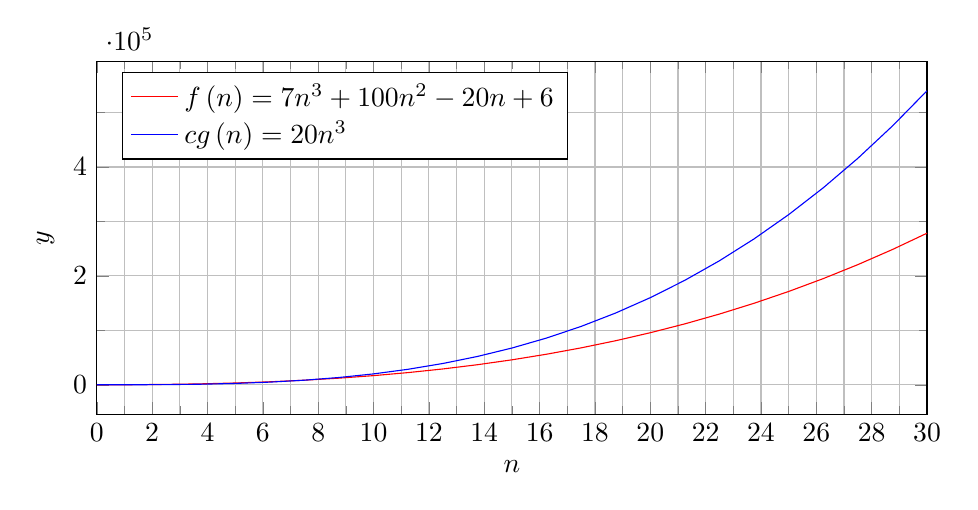
\begin{tikzpicture}
  \begin{axis}[
      xlabel=$n$,
      ylabel=$y$,
      xmin = 0, xmax = 30,
      xtick distance = 2,
      grid = both,
      minor tick num = 1,
      width = \textwidth,
      height = 0.5\textwidth,
      legend cell align = {left},
      legend pos = north west
    ]
    \addplot[domain=0:30,color=red]{7*x^3 + 100*x^2 - 20*x + 6};
    \addplot[domain=0:30,color=blue]{20*x^3};
    \legend{
      $f \left( n \right) = 7n^3 + 100n^2 - 20n + 6$,
      $c g \left( n \right) = 20n^3$
    }
  \end{axis}
\end{tikzpicture}

\subsection{$\Omega$-notation}

\dfn{$\Omega$-notation}{
  Characterizes a lower-bound on the growth rate of a function. I.e. it describes that the function grows no slower than
  a certain rate, based on the highest order term in the function.
}

This means for the same function
\[
  7n^3 + 100n^2 -20n + 6
\]
Its growth rate is $n^3$, and because the function grows no slower than $n^3$, we can say that the function is $\Omega
  \left( n^3 \right) $, and therefore $\Omega \left( n^c \right) $, where $c \leq 3$

\subsubsection{Formal Definition}
\dfn{$\Omega$-notation}{
  For a given function $g \left( n \right) $, we denote by $\Omega \left( g \left( n \right)  \right) $ the set of functions:
  \[
    \Omega \left( g \left( n \right)  \right)  = \{f \left( n \right) : \text{ there exist positive constants $c$ and $n_0$
      such that } 0 \leq c g \left( n \right) \leq f \left( n \right),\, \forall n,\, n \geq n_0   \}
  \]
}

A function $f \left( n \right) $ belongs to the set $\Omega \left( g \left( n \right)  \right) $ if there exists a positive
constant $c$ such that $c g \left( n \right) \leq f \left( n \right)  $ for sufficiently large $n$. This means that the
value of function $f \left( n \right) $ will never be less than the value of $c g \left( n \right) $ for sufficiently large
$n$, where $g \left( n \right) $ is the growth rate of the function.

For example for the function $f \left( n \right) = 7n^3 + 100n^2 - 20n + 6 $, and the order of growth $g \left( n
  \right) = n^3 $. We can say that $f \left( n \right) $ is $\Omega \left( n^3 \right) $ because when $n \geq 6$ and $c =
  1$, $n^3 \leq f \left( n \right) $

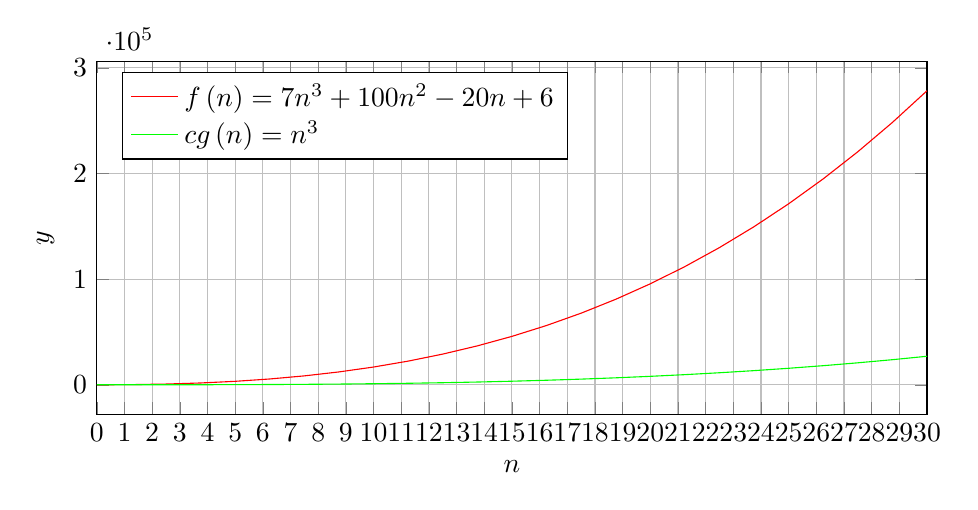
\begin{tikzpicture}
  \begin{axis}[
      xlabel=$n$,
      ylabel=$y$,
      xmin = 0, xmax = 30,
      xtick distance = 1,
      grid = both,
      width = \textwidth,
      height = 0.5\textwidth,
      legend cell align = {left},
      legend pos = north west
    ]
    \addplot[domain=0:30,color=red]{7*x^3 + 100*x^2 - 20*x + 6};
    \addplot[domain=0:30,color=green]{x^3};
    \legend{
      $f \left( n \right) = 7n^3 + 100n^2 - 20n + 6$,
      $c g \left( n \right) = n^3$
    }
  \end{axis}
\end{tikzpicture}

\subsection{$\Theta$-notation}

\dfn{$\Theta$-notation}{
  Characterizes the tight bound on the growth rate of a function. I.e. it describes the precise rate at which the function
  grows based on the highest order term in the function.
}

This notation characterizes the growth rate of a function to within a constant factor from above and below. Therefore if
you can show that a function is both $O \left( n^c \right) $ and $\Omega \left( n^c \right) $, then you have shown that
the function is $\Theta \left( n^c \right) $. I.e for the same function
\[
  7n^3 + 100n^2 -20n + 6
\]
We found that the function is both $O \left( n^3 \right) $ and $\Omega \left( n^3 \right) $, it is also $\Theta \left(
  n^3 \right) $

\subsubsection{Formal Definition}

\dfn{$\Theta$-notation}{
  For a given function $g \left( n \right) $, we denote by $\Theta \left( g \left( n \right)  \right) $ the set of functions:
  \[
    \Theta \left( g \left( n \right)  \right)  = \{f \left( n \right) : \text{ there exist positive constants $c_1$, $c_2$ and $n_0$
      such that } 0 \leq c_1 g \left( n \right) \leq f \left( n \right) \leq c_2 g \left( n \right),\, \forall n,\, n \geq n_0   \}
  \]
}

A function $f \left( n \right) $ belongs to the set $\Theta \left( g \left( n \right)  \right) $ if there exists positive
constants $c_1$ and $c_2$ such that $c_1 g \left( n \right) \leq f \left( n \right) \leq c_2 g \left( n \right)  $ for
sufficiently large $n$. This means that the value of function $f \left( n \right) $ will always be within a constant factor
of the value of $g \left( n \right) $ for sufficiently large $n$, where $g \left( n \right) $ is the growth rate of the function.

For example the function $f \left( n \right) = 7n^3 + 100n^2 - 20n + 6 $, and the order of growth $g \left( n \right) = n^3 $.
We can say that $f \left( n \right) $ is $\Theta \left( n^3 \right) $ because when $n \geq 12$ and $c_1 = 1$ and $c_2 = 20$,

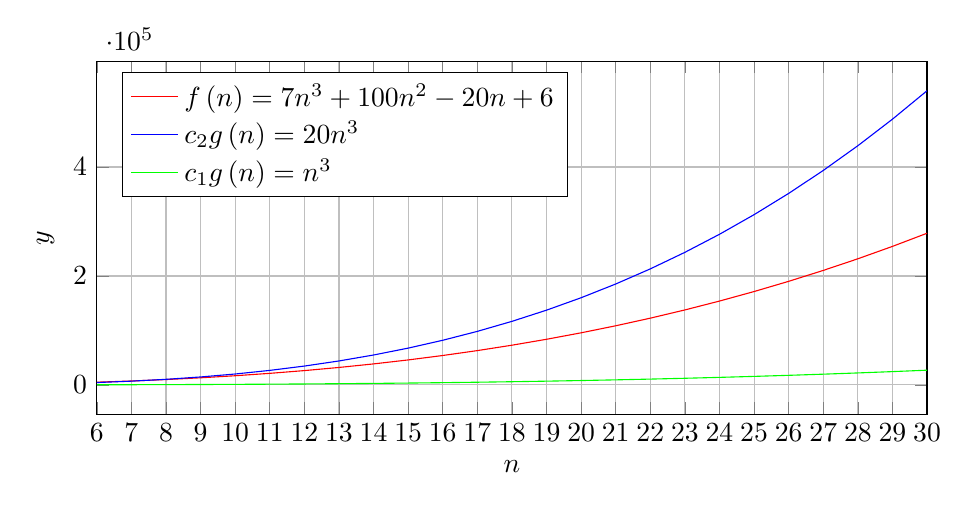
\begin{tikzpicture}
  \begin{axis}[
      xlabel=$n$,
      ylabel=$y$,
      xmin = 6, xmax = 30,
      xtick distance = 1,
      grid = both,
      % minor tick num = 1,
      width = \textwidth,
      height = 0.5\textwidth,
      legend cell align = {left},
      legend pos = north west
    ]
    \addplot[domain=6:30, color=red]{7*x^3 + 100*x^2 - 20*x + 6};
    \addplot[domain=6:30, color=blue]{20*x^3};
    \addplot[domain=6:30, color=green]{x^3};

    \legend{
      $f \left( n \right) = 7n^3 + 100n^2 - 20n + 6$,
      $c_2 g \left( n \right) = 20n^3$,
      $c_1 g \left( n \right) = n^3$
    }
  \end{axis}
\end{tikzpicture}

\subsection{Determining The Running Time of an Algorithm}

Going back to the insertion-sort algorithm we can better characterize its running time using asymptotic notation. Given
that the procedure has nested loops, an outer for loop that always runs $n-1$ times and an inner while loop whose number
of iterations depends on the data being sorted. The while loop variable $j$ starts at $i - 1$ and decreases by 1 each
iteration until it reaches 0 or $A_j \leq \text{key}$. This means the while loop could run $0$ to $i-1$ times. This
means that generally we can deduce an $O \left( n^2 \right) $ running time for the insertion-sort algorithm.

In determining the worst case running time of the insertion sort we need to reiterate that the worst case occurs when
the input is sorted in reverse order. For a value in a reverse sorted array to be inserted into the correct position in
the sub array, it must have been moved in line 4 of the algorithm, and moved $k$ positions. For an element to be moved
$k$ times line 4 needs to have been executed $k$ times. In the worst case where elements need to be moved $i-1$ times
where $i$ is the current index of the element under consideration meaning at least the while loop must be executed $n-1$
times. This means that the worst case running time of the insertion sort is $\Omega \left( n^2 \right) $, because for
every input size $n$ above a certain size $n_0$, there is at least one input of size $n$ that takes at least $cn^2$ time
where $c$ is a positive constant.

Because we have shown that the insertion sort algorithm runs in $O \left( n^2 \right) $ time in all cases, and that
there is an input that takes $\Omega \left( n^2 \right) $ time, we can conclude that the worst-case running time of the
insertion-sort is $\Theta \left( n^2 \right) $

\section{Exercises}

\qs{}{
  Express the function
  \[
    \frac{n^3}{1000} + 100n^2 - 100n + 3
  \]
  in terms of $\Theta$-notation
}

\sol{
  $\Theta \left( n^3 \right) $
}

\qs{}{
  Consider sorting $n$ numbers stored in array $A \left[ 1:n \right] $ by finding the smallest element of $A \left[ 1:n
      \right] $ and exchanging it with the element in $A \left[ 1 \right] $.  Then find the second smallest element of
  $A \left[ 2:n \right] $ and exchange it with $A \left[ 2 \right] $. Continue in this manner for the first $n-1$
  elements of $A$. Write pseudocode for this algorithm, which is known as selection-sort. What loop invariant does this
  algorithm maintain? Why does it need to run for only the first $n-1$ elements, rather than for all $n$ elements? Give
  the best-case and worst-case running times of selection-sort in $\Theta$-notation. Is the best-case running time any
  better?
}

\sol{
  \begin{algorithm}[H]
    \caption{Selection-Sort $\left( A, n \right) $}
    \begin{algorithmic}[1]
      \For{i := 1 to $n -1$}
      \State min := $A_i$
      \State mI := i
      \State j := i
      \While{j $< n - 1$}
      \If{$A_j < \text{ min}$}
      \State min = $A_j$
      \State mI = j
      \EndIf
      \State j = j $+ 1$
      \EndWhile
      \State Swap $A_i$ and $A_{\text{mI}}$
      \EndFor
    \end{algorithmic}
  \end{algorithm}
}


\chapter{Exercises}

\qs{}{
  Describe an algorithm that takes as input a list of $n$ integers and finds the number of negative integers in the list
}

\sol{
  \begin{algorithm}[H]
    \caption{Count-Negative $\left( A,n \right) $}
    \begin{algorithmic}[1]
      \State count := 0
      \For{i := 1 to $n$}
      \If{$A$[i] < $0$}
      \State count = count + 1
      \EndIf
      \EndFor
      \State \Return count
    \end{algorithmic}
  \end{algorithm}
}

\qs{}{
  Describe an algorithm that takes as in put a list of $n$ integers and produces as outputs the largest difference
  obtained by subtracting an integer in the list from the one following it.
}

\sol{
  \begin{algorithm}[H]
    \caption{Largest-Difference $\left( A, n \right) $}
    \begin{algorithmic}[1]
      \State largest := $A_{2} - A_{1}$
      \For{i := 2 to $n - 1$}
      \State diff := $A_{i+1} - A_{i}$
      \If{ diff $>$ largest}
      \State largest = diff
      \EndIf
      \EndFor
      \State \Return largest
    \end{algorithmic}
  \end{algorithm}
}

\qs{}{

}

\sol{
  \begin{algorithm}[H]
    \caption{Repeated-Ints $\left( A, n \right) $}
    \begin{algorithmic}[1]
      \State j := 0
      \State i := 2
      \While{$ i \leq n$}
      \If{$A_i = A_{i-1}$}
      \State j := $j + 1$
      \State $B_j$ := $A_i$
      \Comment{$B$ is the list of repeated values}
      \While{$i \leq n$ and $A_i = C_i$}
      \State i := $i + 1$
      \EndWhile
      \EndIf
      \State i := $i + 1$
      \EndWhile
      \State \Return $B$
    \end{algorithmic}
  \end{algorithm}
}



\end{document}
